% !TEX root = ../thesis.tex

\chapter{Reconstructing Muons in Real Time at the High Luminosity Large Hadron Collider}
\label{chap:TPSAppendix}

\section{Introduction}

% Paragraph about the importance of using muons in the detector
In chapter~\ref{chap:exp}, we explored the main characteristics of the CMS detector, and in particular, the various subsystems devoted to detecting muons that are produced in collision events.
% More about chapter 3 here

In this appendix, we present work towards the implementation of a novel algorithm for reconstructing muon tracks in real time at the LHC.
In section~\ref{sec:CMSUpgrade}, we discuss future upgrades to the CMS detector that will allow for improvements in muon detection in conjunction with the high luminosity upgrades to the LHC.
Later, in section~\ref{sec:TPS}, we introduce the Tracks Plus Stubs algorithm, which will allow for the reconstruction of muon tracks in real time at the L1 trigger level.

\section{Future Upgrades to CMS}
\label{sec:CMSUpgrade}

\section{The Tracks Plus Stubs Algorithm}
\label{sec:TPS}

The upgrades to CMS as described in section~\ref{sec:CMSUpgrade} allow for using the new track trigger to provide the initial information about particle transverse momentum \pt, angular position $\phi$, pseudorapidity $\eta$, and charge $q$.
As muons produced in collision events move throughout the detector, they create detection stubs in the DTs, RPCs, and CSCs, which are L1 trigger primitives that contain information about the angular position $\phi$ and the bending angle $\phi_b$ (only in DTs) in the chamber for which the stub was created.

The Tracks Plus Stubs (TPS) algorithm combines the information from the track trigger and the detection stubs in the chambers to create a candidate track that will later be reconstructed as a muon in the detector.
By using the initial information from the track trigger, the algorithm propagates the initial muon track to the outer layers of the detector.
The propagated values for the angular variables $\phi$ and $\phi_b$ are then compared to those as recorded by the stub measurements.
From this, the algorithm can construct a candidate muon track, which is a combined object consisting of a track from the track trigger, and a collection of stubs associated to the track.

\subsection{Muon Track Propagation}
\label{subsec:prop}

One of the defining characteristics of the CMS detector is the 3.8 T solenoidal magnetic field that is aligned with the beam axis.
In a uniform magnetic field $B$, a charged particle of charge $q$ with momentum transverse to the magnetic field \pt will experience an induced centripetal force due to the Lorentz force that the magnetic field exerts on the charge.
This in turn defines a radius of orbit $R$ for the charge, which is related to the transverse momentum \pt by the relation $\pt=qBR$. It is typical in particle physics to convert the units of the elementary charge so that in terms of $B$ and $R$, we have
\begin{equation}\label{eq:pt}
  \pt=0.3BR\unit{GeV/\clight}.
\end{equation}

However, it is too computationally expensive to use the exact formula for a circular arc in the L1 trigger hardware in order to model the trajectory that a charged particle takes through the detector.
Moreover, the transverse momenta for muons that result in a typical collision event of interest are such that a parabolic approximation is accurate enough to describe the track of the particle.

Assuming that the track starts in the center of the beamline as in Fig.~\ref{fig:arc}, we may approximate the circular arc that the charged particle follows through the detector by
\begin{equation}\label{eq:para}
  y(x)=\frac{x^2}{2R}+bx,
\end{equation}
where $R$ is the radius of curvature as in Eq.~\ref{eq:pt}, and $b$ is a constant to be determined.
First, observe that at the origin, the tangent of the initial angle $\phi_0$ corresponds to the first derivative of~\ref{eq:para} evaluated at $x=0$. Therefore,
\begin{equation}
  \eval{\dv{y}{x}}_{x=0}=\tan\phi_0=b,
\end{equation}
and hence
\begin{equation}
  y(x)=\frac{x^2}{2R}+x\tan\phi_0.
\end{equation}
At the position of the charge $q$, we also have that the tangent of the position angle $\phi$ is given by
\begin{equation}
  \tan\phi=\frac{y(x_\mathrm{stub})}{x_\mathrm{stub}}=\frac{x_\mathrm{stub}}{2R}+\tan\phi_0,
\end{equation}
which we may rearrange to obtain
\begin{equation}
  \tan\phi-\tan\phi_0=\frac{x_\mathrm{stub}}{2R}.
\end{equation}
Since the \pt of a muon that passes through the threshold of the detector is high enough such that the radius $R$ is large, $\Delta\phi\equiv\phi-\phi_0$ is small, and hence we may make the approximation that $\tan\phi-\tan\phi_0\approx\phi-\phi_0$.
Thus,
\begin{align*}\label{eq:phi}
  \phi &= \frac{x_\mathrm{stub}}{2R}+\phi_0\\
  &= ck+\phi_0,
  \numberthis
\end{align*}
where we have used the fact that $k=1/R$ and $c$ is a constant to be determined based on the position of the stub.
Furthermore, in Fig.~\ref{fig:arc}, we can see that due to the symmetry of the circular arc traced by the track of the particle, the bending angle $\phi_b$ must be equal to the change in the position angle $\Delta\phi$, and hence we immediately obtain
\begin{equation}\label{eq:phib}
  \phi_b=ck.
\end{equation}

\begin{figure}[htbp]
  \centering
  % !TEX root = ../../thesis.tex
\begin{tikzpicture}
  % Axes
  \draw[->] (0,0) -- (2,0) node[below] {$x$};
  \draw[->] (0,0) -- (0,2) node[left] {$y$};

  % Arc
  \coordinate (q) at ($(120:5)+(15:5)$);
  \draw[fill=black] (120:5) circle (1pt);
  \draw[red] (0,0) arc (-60:15:5);
  \draw[->,thick,red] (q) -- ($(q)+(105:1)$) node[left,red] {$\vb{p}_\mathrm{T}$};
  \draw[red,dashed] (0,0) -- (30:2);

  % Lines
  \draw[dashed] (0,0) -- (120:5) node[pos=0.5,left] {$R$};
  \draw[dashed] (120:5) -- (q) node[pos=0.5,above] {$R$};
  \draw[dashed] (67.5:3.044) -- ($(120:5)+(-22.5:5)$) node[pos=0.5,above] {$s$};

  % Angles
  \draw[red] (0.75,0) arc (0:30:0.75) node[pos=0.75,right,red] {$\phi_0$};
  \draw[cyan] (0.5,0) arc (0:67.5:0.5) node[pos=0.8,above right,cyan] {$\phi$};
  \draw (30:1.25) arc (30:67.5:1.25) node[pos=0.8,above right] {$\Delta\phi$};
  \draw[cyan,dashed] (q) -- ($(q)+(67.5:1)$);
  \draw[red] ($(q)+(67.5:0.5)$) arc (67.5:105:0.5) node[pos=0.35,above,red] {$\phi_b$};

  % Charge
  \draw[cyan] (0,0) -- (q) node[pos=0.5,left,cyan] {$L$}; % 6.088
  \draw[fill=cyan] (q) circle (2.5pt) node [right,cyan] {$q$};
  \draw ($(q)+(1.25,-0.5)$) node {$(x_\mathrm{stub},y_\mathrm{stub})$};
\end{tikzpicture}

  \caption{Illustration of the circular trajectory taken by a particle with charge $q$ positioned at $(x_\mathrm{stub},y_\mathrm{stub})$ in a uniform magnetic field. The track starts at the origin with an initial angle $\phi_0$ tangent to the track of the particle, and ends with a final angle of $\phi$ for a total change in angle $\Delta\phi\equiv\phi-\phi_0$. The charged particle covers a radial distance $L$ with respect to the origin of the track, and the perpendicular distance between the mid-point of the track and the radial line $L$ is denoted by the sagitta $s$. The vector corresponding to the \pt of the charge is labeled, with the bending angle $\phi_b$ drawn with respect to the radial line $L$.}
  \label{fig:arc}
\end{figure}

With equations~\ref{eq:phi} and~\ref{eq:phib} in hand, we may now propagate the tracks based on the initial information about the curvature $k$ and angle $\phi_0$.
The CMS detector consists of multiple layers of detection chambers, each chamber requires its own propagation constant $c(\eta,d)$, as the relevant variables to consider for $c$ based on the geometry of the detector is the pseudorapidity of the track $\eta$ and the station depth $d$.
Rather than obtaining these constants analytically, they are obtained by using simulation data. % Elaborate on the simulation samples used later

To do this, we divide the detector into separate $\eta$ regions and depths, and treat each section as a separate detector with its own propagation constant $c(\eta,d)$.
We then look at two-dimensional histograms of $\Delta\phi$ and $\phi_b$ from simulated detection stubs as functions of $k$ for each section of the detector based on simulated detection stubs.
An example of this can be seen in Fig.~\ref{fig:deltaPhiHist}.
For every bin in curvature $k$, the distribution of $\Delta\phi$ or $\phi_b$ is roughly Gaussian, and hence we fit Gaussians to the vertical slices of these histograms.
We then consider the mean of these Gaussians and make linear fits for $\Delta\phi$ and $\phi_b$ in accordance with equations~\ref{eq:phi} and~\ref{eq:phib}.
These then define the propagation constants $c(\eta,d)$ for each detector, thereby allowing us to predict where a muon produced at the beamline during a collision event will end up in the detection chambers.

\begin{figure}[htbp]
  \centering
  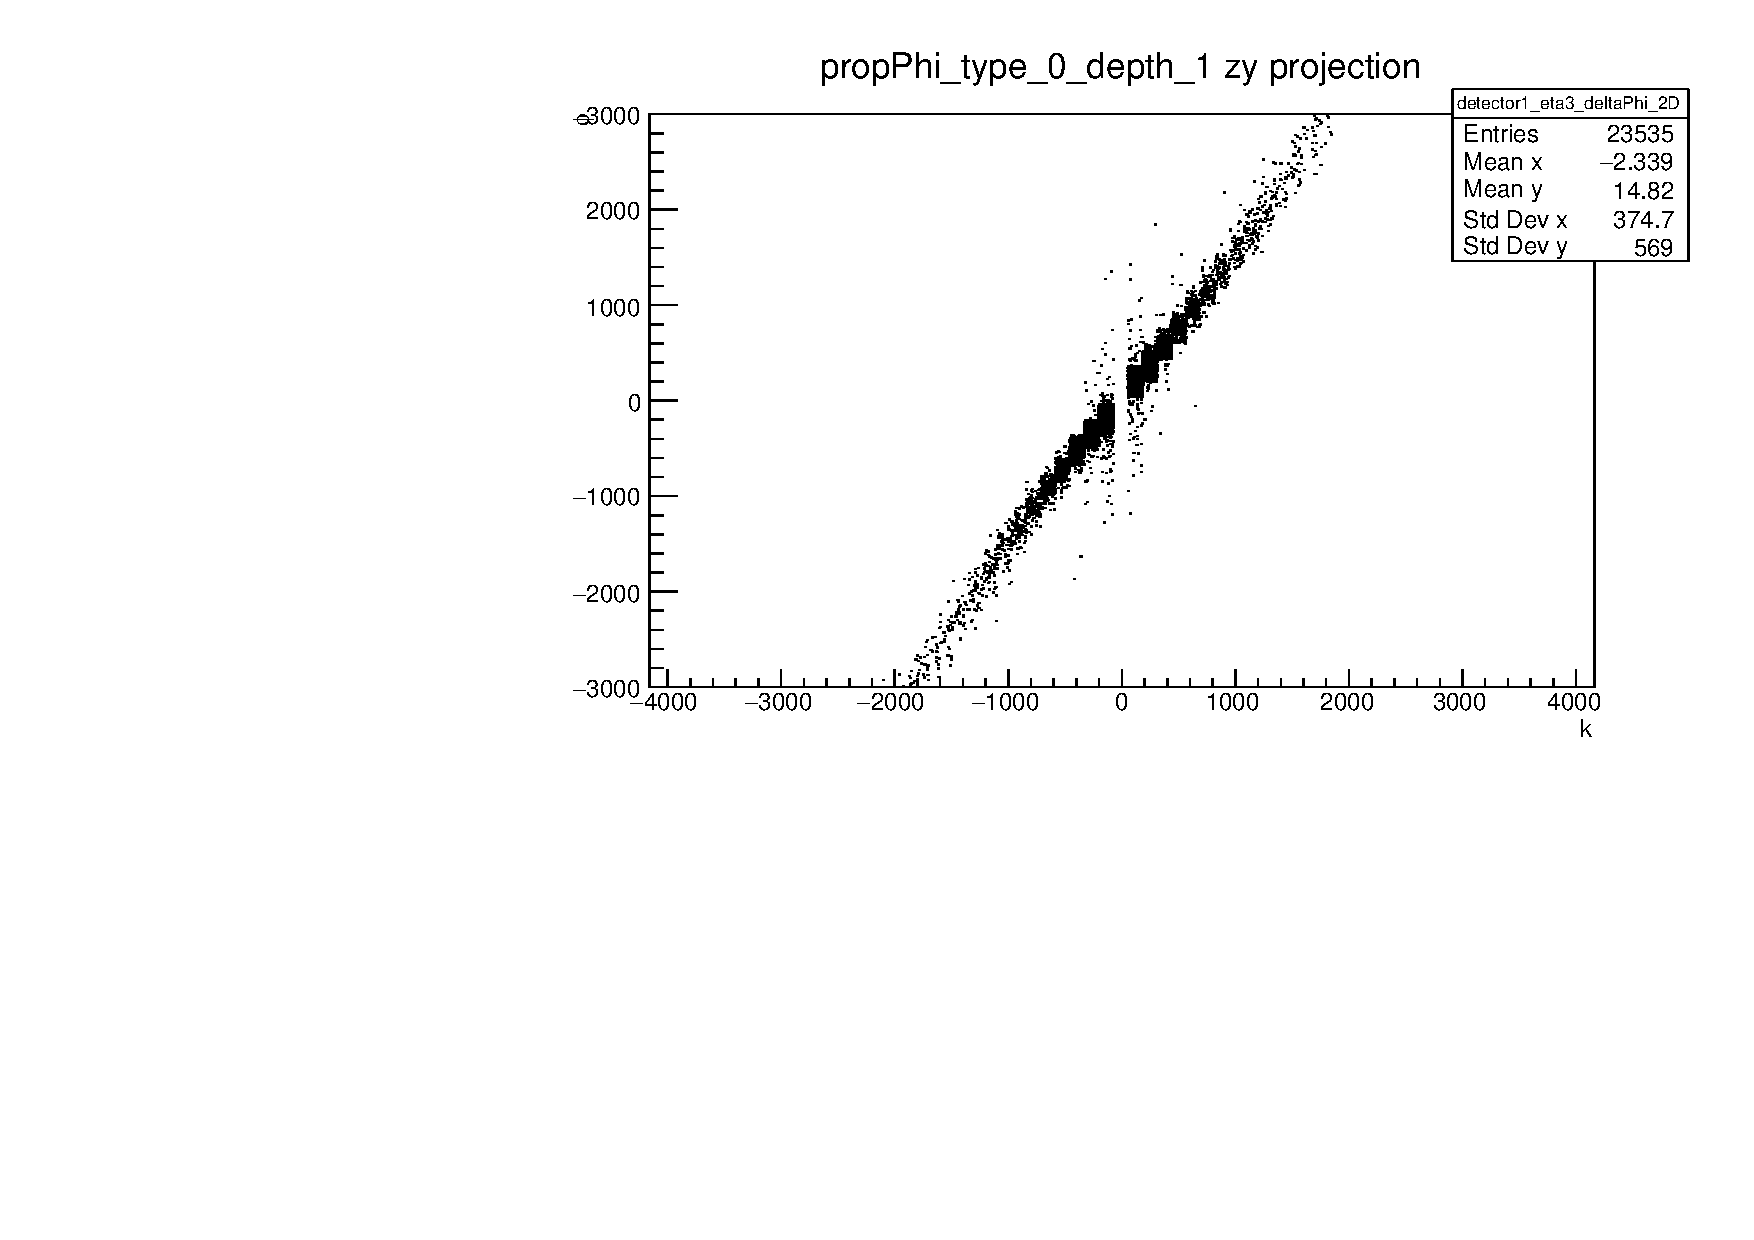
\includegraphics[width=0.48\textwidth]{fig/TPS/deltaPhi_2D.pdf}
  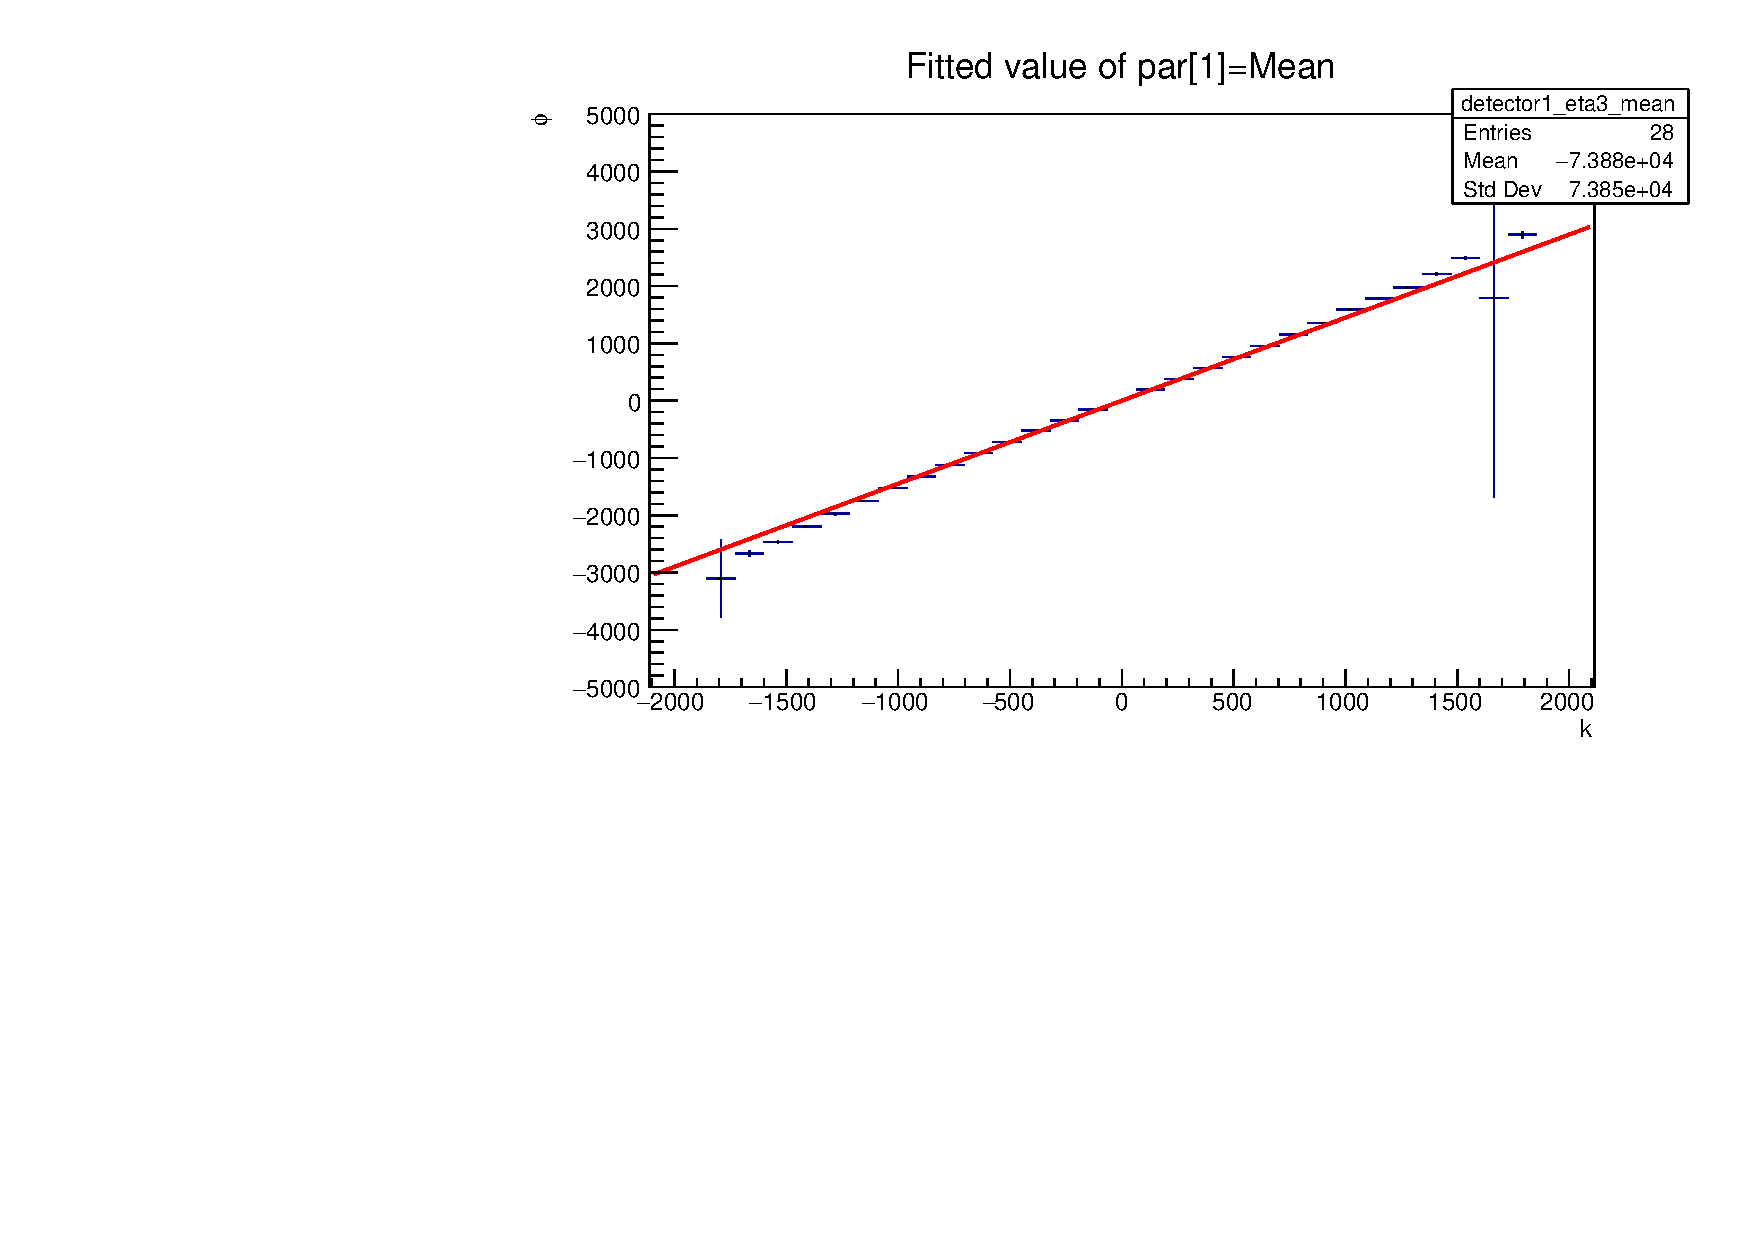
\includegraphics[width=0.48\textwidth]{fig/TPS/deltaPhi_mean.pdf}
  \caption{Two-dimensional distribution of $\Delta\phi$ from simulated detection stubs as a function of curvature $k$ (left), and linear fit for the mean values of Gaussians fitted to the vertical slices of the two-dimensional histogram (right). Propagation constants $c(\eta,d)$ for $\Delta\phi$ and $\phi_b$ for each section of the detector are obtained through these linear fits, in accordance with equations~\ref{eq:phi} and~\ref{eq:phib}.}
  \label{fig:deltaPhiHist}
\end{figure}

\subsection{Pull Distributions and Stub Matching}
\label{subsec:pulls}

Once the propagation constants are obtained, the information for a candidate muon obtained from the track trigger can be used to predict where the muon detection stubs will be found in the detector based on the initial information about the curvature of the track $k$ and the initial angle $\phi_0$.
One of the main considerations in matching a track to detection stubs is the position resolution for the stub measurements.
The standard deviation of the Gaussian fits for $\Delta\phi$ and $\phi_b$ as described in the previous subsection corresponds to the position resolution of the measurements, and has a quadratic form
\begin{equation}
  \sigma=\sqrt{\alpha k^2+\beta},
\end{equation}
where $\alpha$ is a multiple scattering term that dominates for high curvature tracks (i.e., low $p_\mathrm{T}$ tracks), and $\beta$ is a constant term corresponding to the position uncertainty of the detector.

However, this form for $\sigma$, as with the analytic forms for the propagated $\phi$ and $\phi_b$ values, is too computationally expensive to implement into the hardware.
Instead, we approximate the position resolution using
\begin{equation}\label{eq:posRes}
  \sigma\approx a|k|+b,
\end{equation}
where $a$ and $b$ are constants analogous to $\alpha$ and $\beta$.
Fig.~\ref{fig:deltaPhiRes} shows an example of the position resolution from one of the Gaussian fits for $\Delta\phi$ and the fit obtained for equation~\ref{eq:posRes}.
As with the propagation coefficients $c(\eta,d)$, the position resolution constants $a(\eta,d)$ and $b(\eta,d)$ are also specific to each detector based on the $\eta$ region and depth.

\begin{figure}[htbp]
  \centering
  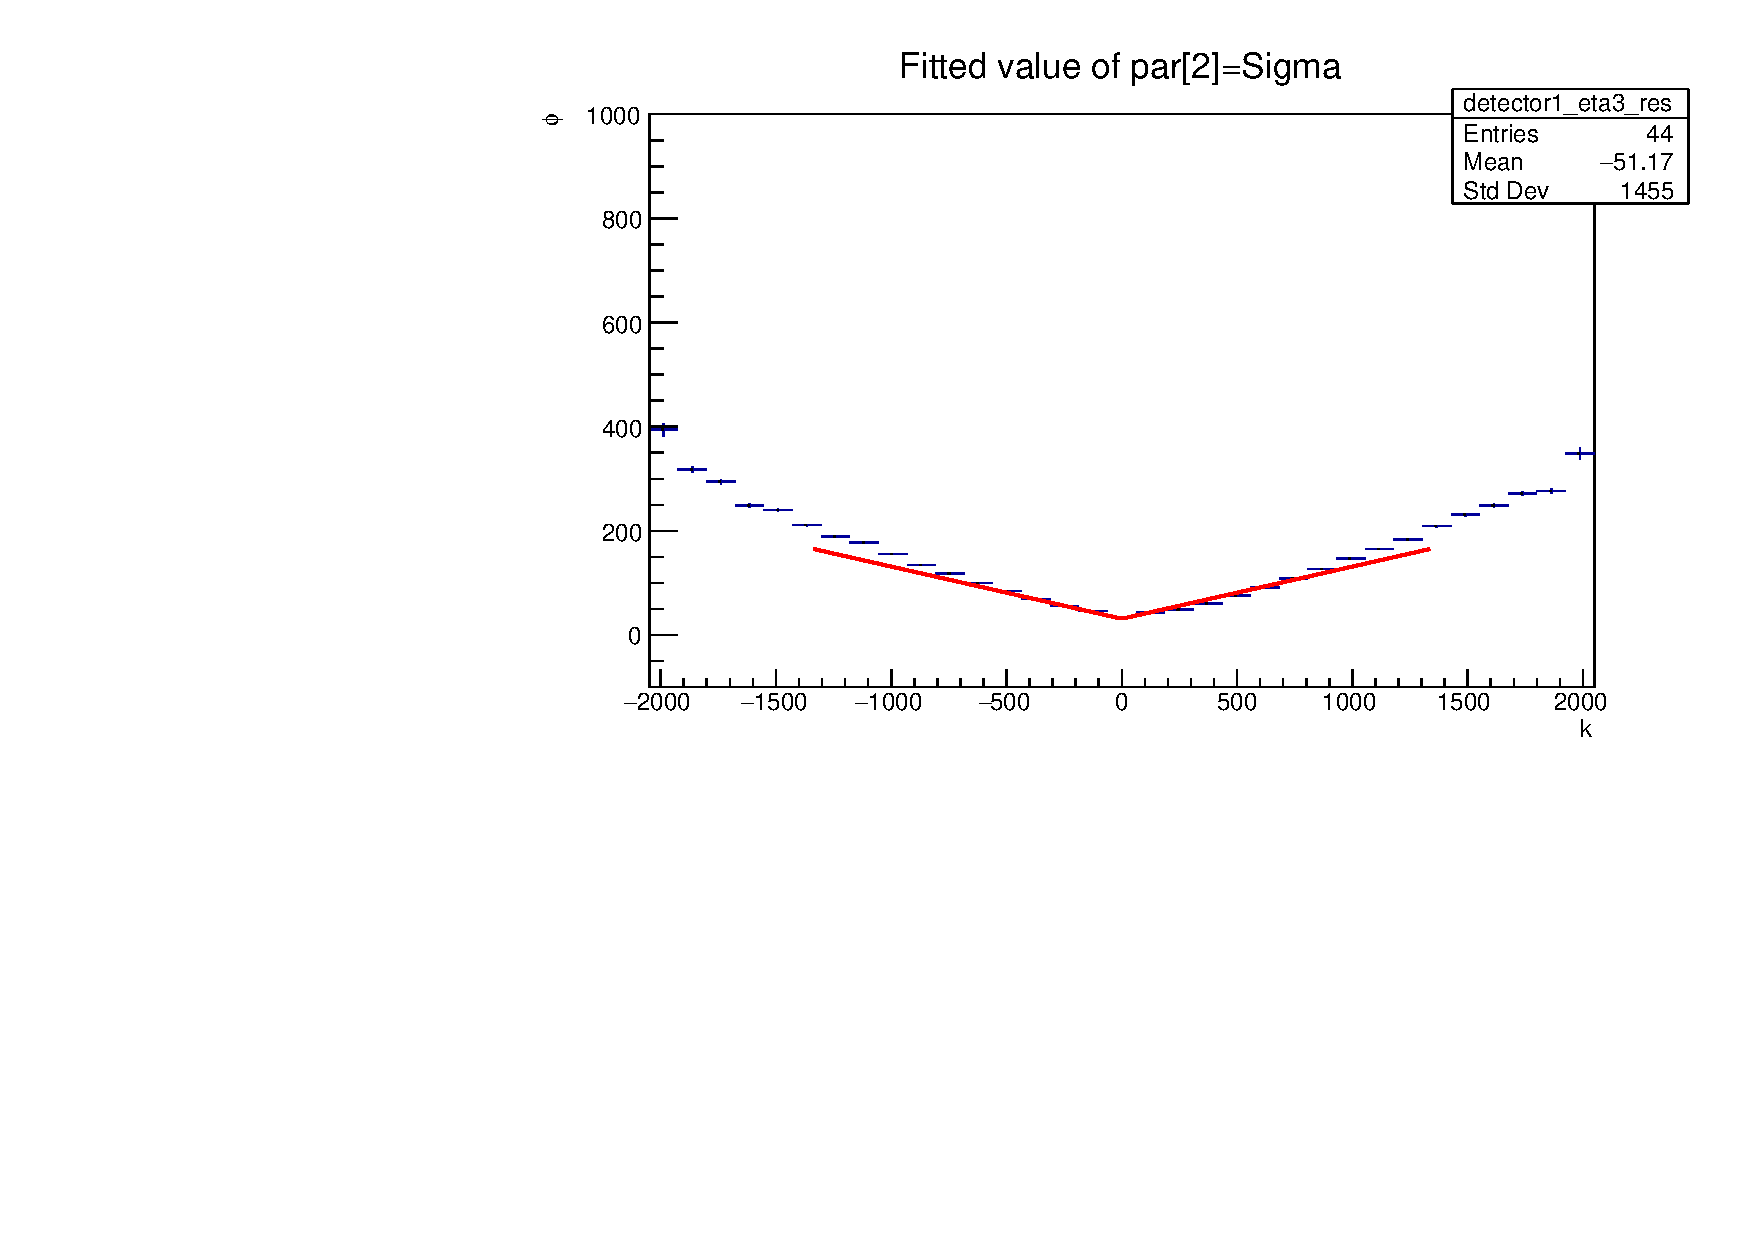
\includegraphics[width=0.48\textwidth]{fig/TPS/deltaPhi_res.pdf}
  \caption{}
  \label{fig:deltaPhiRes}
\end{figure}

With the means to propagate the tracks from the track trigger and determine the resolution of the stub measurements, we may now proceed with determining whether or not a stub is suitable for being matched with a candidate muon.
To do this, we consider the pull distributions for each stub with respect to a track.
For each track, we check the pull values of every stub that may get matched with the track, which are given by
\begin{equation}
  P_\phi=\frac{\phi_\mathrm{prop}-\phi_\mathrm{stub}}{\sigma}=\frac{\phi_\mathrm{prop}-\phi_\mathrm{stub}}{a|k|+b}.
\end{equation}
The distributions made by sampling these pull values from simulation are Gaussian distributed, and an example may be seen in Fig.~\ref{fig:deltaPhiPull}.
We then match stubs to tracks by considering the absolute value of the pulls for each stub.
If $|P_\phi|$ for a stub is below a certain threshold for a track, then the stub will be matched to the track.
Stubs that exceed the threshold for $|P_\phi|$ will instead be discarded.

\begin{figure}[htbp]
  \centering
  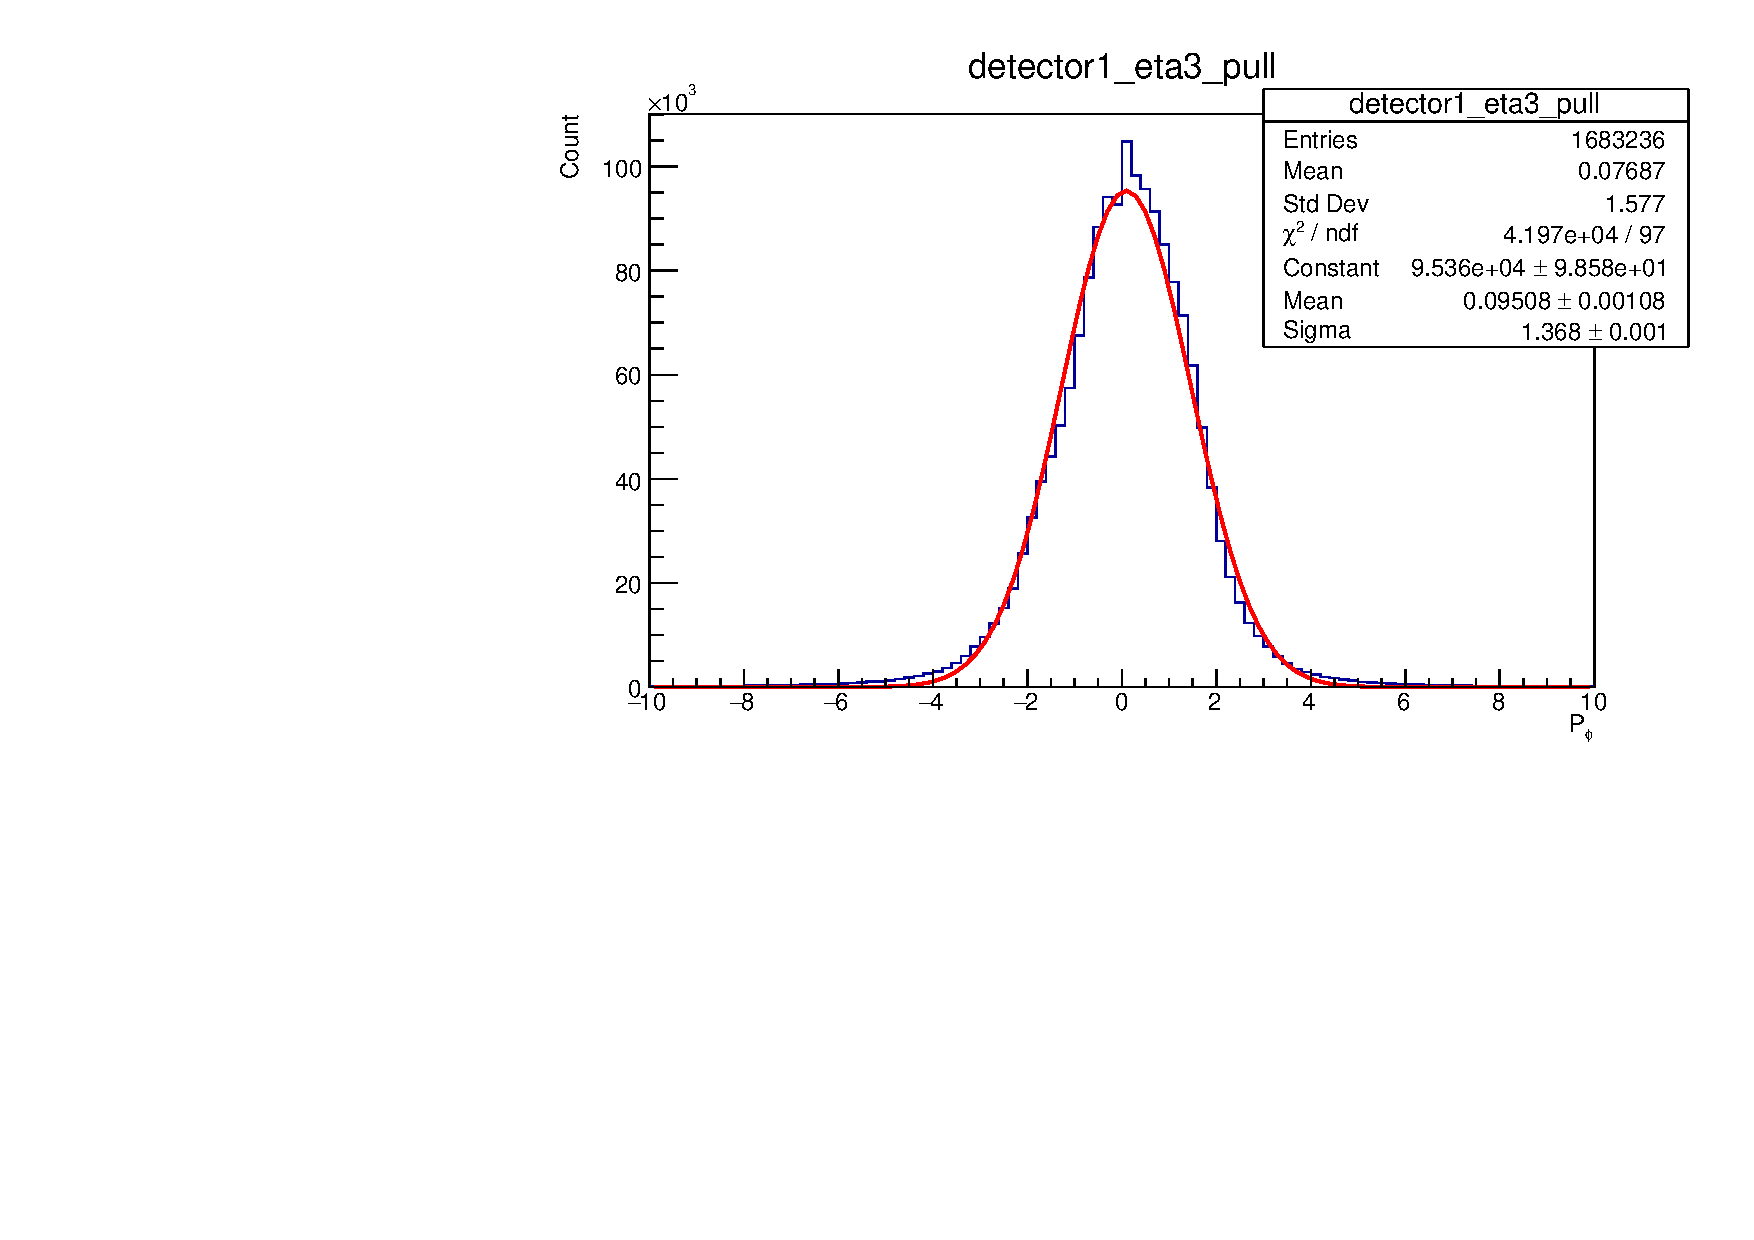
\includegraphics[width=0.48\textwidth]{fig/TPS/deltaPhi_pull.pdf}
  \caption{}
  \label{fig:deltaPhiPull}
\end{figure}


\subsection{Track Cleaning and Isolation}
\label{subsec:cleaning}

\begin{figure}[htbp]
  \centering
  % !TEX root = ../../thesis.tex
\begin{tikzpicture}
  % Tracks Case 1
  \draw[red] (0,0) arc (-80:-20:3);
  \draw[orange] (0,0) arc (-100:-10:3.5);

  % Tracks Case 2
  \draw[red] (8,0) arc (-80:-10:3.25);
  \draw[orange] (8,0) arc (-100:-10:3.5);

  % Stubs Case 1
  \draw[fill=black] (10:1) circle (1pt);
  \draw[fill=black] (16:2) circle (1pt);
  \draw[fill=black] (22:3) circle (1pt);
  \draw[fill=black] (28:4) circle (1pt);

  % Stubs case 2
  \draw[fill=black] ($(8,0)+(7:1)$) circle (1pt);
  \draw[fill=black] ($(8,0)+(12:2)$) circle (1pt);
  \draw[fill=black] ($(8,0)+(20:3)$) circle (1pt);
  \draw[fill=black] ($(8,0)+(27:4)$) circle (1pt);

  % Labels Case 1
  \draw (2,3.25) node {Case 1:};

  \draw[red,->] (0,1) -- (10:1);
  \draw[red,->] (0,1) -- (16:2);
  \draw (0,1) node[red,fill=white,inner sep=2pt] {Track 1 Stubs};

  \draw[orange,->] (4,0) -- (10:1);
  \draw[orange,->] (4,0) -- (16:2);
  \draw[orange,->] (4,0) -- (22:3);
  \draw[orange,->] (4,0) -- (28:4);
  \draw (4,0) node[orange,fill=white,inner sep=2pt] {Track 2 Stubs};

  % Labels Case 2
  \draw (10,3.25) node {Case 2:};

  \draw[red,->] (8,1) -- ($(8,0)+(7:1)$);
  \draw[red,->] (8,1) -- ($(8,0)+(12:2)$);
  \draw[red,->] (8,1) -- ($(8,0)+(20:3)$);
  \draw[red,->] (8,1) -- ($(8,0)+(27:4)$);
  \draw (8,1) node[red,fill=white,inner sep=2pt] {Track 1 Stubs};

  \draw[orange,->] (12,0) -- ($(8,0)+(7:1)$);
  \draw[orange,->] (12,0) -- ($(8,0)+(12:2)$);
  \draw[orange,->] (12,0) -- ($(8,0)+(20:3)$);
  \draw[orange,->] (12,0) -- ($(8,0)+(27:4)$);
  \draw (12,0) node[orange,fill=white,inner sep=2pt] {Track 2 Stubs};
\end{tikzpicture}

  \caption{}
  \label{fig:clean}
\end{figure}

\begin{figure}[htbp]
  \centering
  % !TEX root = ../../thesis.tex

\begin{tikzpicture}
  % Axis
  \draw[->] (0,0) -- (8,0) node[right] {$z$};

  % Tracks
  \draw[fill=black] (1,0) circle (1pt);
  \draw[fill=black] (3.5,0) circle (1pt);
  \draw[fill=black] (4,0) circle (1pt);
  \draw[fill=black] (7,0) circle (1pt);
  \draw[->,thick] (1,0) -- ($(1,0)+(105:2)$);
  \draw[->,thick] (3.5,0) -- ($(3.5,0)+(75:3)$);
  \draw[->,thick] (4,0) -- ($(4,0)+(110:3.5)$) node[above] {TPS $\mu$};
  \draw[->,thick] (7,0) -- ($(7,0)+(80:2.5)$);

  % Cone
  \draw[rotate around={20:(4,0)},dotted] (4,2) ellipse (1.3 and 0.6);
  \draw[rotate around={20:(4,0)},dotted] (4,0) -- ($(4,0)+(55.725:2.25)$);
  \draw[rotate around={20:(4,0)},dotted] (4,0) -- ($(4,0)+(124.275:2.25)$);

  % Labels
  \draw[|-|] (3.5,-0.25) -- (4,-0.25) node[below] {$|dz|<0.2$ cm};
  \draw (5.5,2.75) node {$\Delta R=0.5$};
\end{tikzpicture}

  \caption{}
  \label{fig:isol}
\end{figure}

\subsection{Trigger Efficiencies and Rates}
\label{subsec:rates}

\section{Results and Future Implementation}
\label{subsec:TPSResults}
